% \newcommand{\path}{../..}
\newcommand{\pathGraphics}{figures/} % path figures

% pdflatex -ini -job="2020_21_gfif_zahlensysteme_header_compiled" "&pdflatex 2020_21_gfif_zahlensysteme_header.tex\dump"

% \documentclass[a4paper,11pt,twoside]{article} % landscape
% \usepackage{a4wide}

%\documentclass[twoside]{article}
\documentclass[a4paper,11pt,twoside]{article}
\usepackage{a4wide}


%\usepackage[german]{babel}
\usepackage[utf8]{inputenc}
\usepackage{amsmath,amssymb}
\usepackage{graphicx}
\usepackage{wrapfig} % wrap text around figures
\usepackage{fancyhdr} % for a fancy header and footer
\usepackage{datetime}
\usepackage{color}
\usepackage{float} %without it, tables position more or less random, with this an writing \begin{table}[H] the table appears right where it is defined!
\usepackage[table,xcdraw]{xcolor}

\usepackage{tabularx}
\usepackage{multicol}

\usepackage{subcaption} % for subfigures

\usepackage[symbol]{footmisc} % footnote: use symbols instead numbers

\usepackage{enumitem}

\usepackage{amsthm}
\usepackage{bm}

\newcommand{\sectionnumbering}[1]{% to swich to roman pagenumbering at abstract and table of content
  \setcounter{section}{0}%
  \renewcommand{\thesection}{\csname #1\endcsname{section}}}

\usepackage{verbatim} % for multiple line comments; \begin{comment} write comment \end{comment}

\usepackage{tikz} %use for tikzpicture to draw lines usw
\usetikzlibrary{backgrounds,angles,quotes}
\usepackage{tkz-euclide} % http://mirror.easyname.at/ctan/macros/latex/contrib/tkz/tkz-euclide/doc/TKZdoc-euclide.pdf
\usepackage{tikz-3dplot}
\usetikzlibrary{babel}
%\usetkzobj{all} %%% IMPORTANT ATTENTION: Commented this out when switching Windows -> Mac

%\usepackage{lipsum}

\usepackage{siunitx} % for writing numbers with units
% e.g. \SI{6.3e8}{km}, \ang{62.59}, \num{100}'s \si{km}, \SI{53}{\degree}

\usepackage{exsheets} %http://mirror.switch.ch/ftp/mirror/tex/macros/latex/contrib/exsheets/exsheets_en.pdf
%\usepackage{tasks} % needs not be loaded if 'exsheets' is loaded (is part of exsheets). for typical ordering of math exercises, https://www.ctan.org/tex-archive/macros/latex/contrib/tasks?lang=de


% tables
\usepackage{multirow} % multirows in tables
\usepackage{booktabs}
%\usepackage{savefnmark}
%\usepackage{fmtcount}

\usepackage{adjustbox} % rotate stuff

\usepackage{polynom} % polynomdivision usw

\usepackage{pgf,tikz}
\usepackage{mathrsfs}\usetikzlibrary{arrows}
\usepackage{pgfplots} % for plotting fcns e.g. arcsin...

\usepackage{tagging}

% to show lines for handwriting
\usepackage{pgffor, ifthen}
\newcommand{\notes}[3][\empty]{%
    \noindent \vspace{10pt}\\
    \foreach \n in {1,...,#2}{%
        \ifthenelse{\equal{#1}{\empty}}
            {\rule{#3}{0.5pt}\\}
            {\rule{#3}{0.5pt}\vspace{#1}\\}
        }
}
% create empty space to solve exercises:
%
\newcommand{\notesempty}[2][\empty]{%
    \noindent \vspace{10pt}\\
    \foreach \n in {1,...,#2}{%
        \ifthenelse{\equal{#1}{\empty}}
            {\\}
            {\vspace{#1}\\}
        }
}

\usepackage{hyperref}   % Hyperlinks
\usepackage{cleveref}

\graphicspath{\pathGraphics}

\usepackage{circuitikz}
\usetikzlibrary{intersections}
%\usepackage{qrcode}
\pgfplotsset{compat=1.16}

\usepackage[ngerman]{babel}


\usepackage{cprotect} % use \cprotEnv in front of question/solution if want to use code listing in it

\usepackage{nbaseprt} % for hexadecimal numbers, https://mirror.kumi.systems/ctan/macros/latex/contrib/numprint/nbaseprt.pdf
%\nplpadding{6} % add for padding: 
\npthousandsep{}
\npdecimalsign{.}
\nprounddigits{0}

% some commands
\def\ba#1\ea{\begin{align}#1\end{align}}
\def\bas#1\eas{\begin{align*}#1\end{align*}}
\def\bmat#1\emat{\begin{pmatrix}#1\end{pmatrix}}
\def\btasks#1\etasks{\begin{tasks}#1\end{tasks}}
\newcommand{\ve}[1]{\vec{#1}}
\newcommand{\veTwo}[2]{\begin{pmatrix}#1\\#2\end{pmatrix}}
\newcommand{\veThree}[3]{\begin{pmatrix}#1\\#2\\#3\end{pmatrix}}
\newcommand{\veFour}[4]{\begin{pmatrix}#1\\#2\\#3\\#4\end{pmatrix}}
\newcommand{\ora}[1]{\overrightarrow{#1}}
\newcommand{\ola}[1]{\overleftarrow{#1}}
\newcommand{\s}[1]{\sqrt{#1}}

\def \bit{\begin{itemize}\setlength\itemsep{0em}} %\vspace{-5mm}
\def \eit{\end{itemize}}

\def \ben{\begin{enumerate}\setlength\itemsep{0em}} %\vspace{-5mm}
\def \een{\end{enumerate}}

\def \N{\mathbb{N}}
\def \Z{\mathbb{Z}}
\def \Q{\mathbb{Q}}
\def \R{\mathbb{R}}
\def \C{\mathbb{C}}

\def \ra{\rightarrow}
\def \longra{\longrightarrow}
\def \Ra{\Rightarrow}
\def \Longra{\Longrightarrow}
\def \la{\leftarrow}
\def \longla{\longleftarrow}
\def \La{\Leftarrow}
\def \Longla{\Longleftarrow}

\def \lra{\leftrightarrow}
\def \longlra{\longleftrightarrow}
\def \Lra{\Leftrightarrow}
\def \Longlra{\Longleftrightarrow}

\def \ssm{\smallsetminus}
\def \sm{\setminus}
\def \ol{\overline}

\def \l{\left}
\def \r{\right}

\def \a{\alpha}
\def \b{\beta}
\def \g{\gamma}

\def \c{\cdot}

\def \el{\in}
\def \notel{\notin}

\newcommand{\f}{\frac}

\def \q{\quad}
\newcommand{\p}{\phantom}

\def\bs#1\es{\begin{split}#1\end{split}}

\def \L{\mathbb{L}}

\newcommand{\grid}[1]{
    \begin{figure}[H]
        \centering
        \begin{tikzpicture}[scale=1]
        \draw[step=0.5,gray,very thin,solid] (-0,2,-0.2) grid (\textwidth,#1);
        \end{tikzpicture}
    \end{figure}
}

\newcommand{\lpsus}[2]{
    \ifdraft\color{blue}#1\color{black}
    \else#2\fi
}

%\newcommand{\lp}[1]{
%    \ifdraft\color{blue}#1\color{black}
%    \else\fi
%}
%
%\newcommand{\sus}[1]{
%    \ifdraft
%    \else#1\fi
%}

\newcommand{\ca}{\centering\arraybackslash} % for tables, to center content


% old commands (from thesis):
%\def\baa#1\eaa{\begin{align*}#1\end{align*}}
%\newcommand{\f}{\frac}
%\newcommand{\p}{\partial}
%\newcommand{\be}{\begin{eqnarray}}
%\newcommand{\ee}{\end{eqnarray}}
%\newcommand{\bea}{\begin{eqnarray*}}
%	\newcommand{\eea}{\end{eqnarray*}}
%\newcommand{\s}[2]{\sum_{#1}^{#2}}
%
%\def\bsub#1\esub{\begin{subequations}#1\end{subequations}}



%\def \k{\kappa}

%\def \A{\mathcal{A}}
%\def \B{\mathcal{B}}
%\def \F{\mathcal{F}}
%\def \I{\mathcal{I}}
%\def \V{\mathcal{V}}
%\def \U{\mathcal{U}}
%\def \K{\mathcal{K}}

%\def \E{\mathfrak{E}}
%\def \J{\mathfrak{J}}
%\def \G{\mathfrak{G}}

%\def \m{\mu}
%\def \n{\nu}
%\def \nab{\nabla}
%\def \cov{\nabla}
%\def \P{\Phi}
%\def \O{\Omega}
%\def \a{\alpha}
%\def \b{\beta}
%\def \g{\gamma}
%\def \lam{\lambda}
%\def \eps{\epsilon}

%\def \t{\text}


%\def \ra{\rightarrow}
%\def \R{\mathds{R}}

%\def \barP{\bar{\Phi}}
%\def \barf{\bar{f}}
%\def \barg{\bar{g}}
%\def \bargamma{\bar{\gamma}}
%\def \barF{\bar{\mathcal{F}}}
%\def \bargamma{\bar{\gamma}}

%\newcommand{\new}[1]{{\color{blue}\ensuremath{\blacktriangleright$#1$\blacktriangleleft}}}
%\newcommand{\correction}[1]{{\color{red}\ensuremath{\blacktriangleright$#1$\blacktriangleleft}}}

%\newcommand{\order}[2]{\mathcal{O}\left(#1^#2\right)}






% \def \Epsilon{\mathcal{E}}

%------------------------------------------
%------------------------------------------
% INPUT
\newcommand{\teacher}{Andreas Schärer \& Moritz Küng}
\newcommand{\teachershort}{sca,kng}
\newcommand{\mail}{sca@ksr.ch,kng@ksr.ch}
\newcommand{\class}{1M}
\newcommand{\datum}{2021}
\newcommand{\courseDE}{GF Informatik}
% \newcommand{\courseEN}{Mathematics}
\newcommand{\topicDE}{Zahlensysteme}
% \newcommand{\topicEN}{Functions II}

% define my exercise
\newcounter{aufgabe} % start counter
\setcounter{aufgabe}{1}

\setlength{\parindent}{0pt} % offset on RHS (if 0, no indent)
\setlength{\parskip}{15pt} % distance btw exercise title and the exercise text, and next exercise title

\renewcommand{\d}{\mathrm{d}}
\newcommand{\mynewex}[1]{
{\bf Exercise \theaufgabe}
\stepcounter{aufgabe} #1 }

%\topmargin-10mm % decrease top margin (less distance btw top edge of sheet and txt)


%
% Define colors
\definecolor{myblue}{rgb}{0.1875,0.503906,0.929688}
\definecolor{myorange}{rgb}{1,0.54902,0}

\usepackage[
    margin=1.0in,
    bottom=1in,
    top=1.8cm,
    headsep=0.5cm
    ]{geometry}

\fancypagestyle{mypagestyle}{%
  \fancyhf{}% Clear header/footer
  \fancyhead[OL]{\class/\teachershort} %on Odd page, right
  \fancyhead[EL]{\class/\teachershort } %on Even page, left
  \fancyhead[OR]{\datum} % Title on Even page, right
  \fancyhead[ER]{\datum}% Title on Even page, Centred
  \fancyfoot[C]{\thepage}%
  \fancyfoot[R]{v: \ddmmyyyydate\today}%
  \renewcommand{\headrulewidth}{.4pt}% Header rule of .4pt
}
\pagestyle{mypagestyle}


\usepackage[framemethod=TikZ]{mdframed}
%\usepackage[framemethod=default]{mdframed}
% for auto-split frame environment, load after amsthm
%http://www.pirbot.com/mirrors/ctan/macros/latex/contrib/mdframed/mdframed.pdf

\newcounter{definition}[section]
\renewcommand{\thedefinition}{\thesection.\arabic{definition}}

\newcounter{theorem}[section]
\renewcommand{\thetheorem}{\thesection.\arabic{theorem}}

\newcounter{assignment}[section]
\renewcommand{\theassignment}{\thesection.\arabic{assignment}}

\newcounter{auftrag}[section]
\renewcommand{\theauftrag}{\thesection.\arabic{auftrag}}

\newcounter{example}[section]
\renewcommand{\theexample}{\thesection.\arabic{example}}

%\newenvironment{example}[1][]{%
%    \refstepcounter{example}
%    \textbf{Example~\theexample:\\#1}
%}


\newenvironment{definition}[1][]{%
    \refstepcounter{definition}
    \begin{mdframed}[%
        frametitle={Definition~\thedefinition\ #1},
        linecolor=myorange,
        skipabove=\baselineskip plus 2pt minus 1pt,
        skipbelow=\baselineskip plus 2pt minus 1pt,
        linewidth=0.8pt,
        splittopskip=30pt,
        splitbottomskip=30pt
%        frametitlerule=true
%        frametitlebackgroundcolor=gray!30
    ]%
}{%
    \end{mdframed}
}

\newenvironment{theorem}[1][]{%
    \refstepcounter{theorem}
    \begin{mdframed}[%
        frametitle={Theorem~\thetheorem\ #1},
        linecolor=green,
        skipabove=\baselineskip plus 2pt minus 1pt,
        skipbelow=\baselineskip plus 2pt minus 1pt,
        linewidth=0.8pt,
        splittopskip=30pt,
        splitbottomskip=30pt
%        frametitlerule=true
%        frametitlebackgroundcolor=gray!30
    ]%
}{%
    \end{mdframed}
}

% ENGLISH

\newenvironment{assignment}[1][]{%
    \refstepcounter{assignment}
    \begin{mdframed}[%
        frametitle={Task~\theassignment\ #1},
        linecolor=blue,
        skipabove=\baselineskip plus 2pt minus 1pt,
        skipbelow=\baselineskip plus 2pt minus 1pt,
        linewidth=0.8pt,
        splittopskip=30pt,
        splitbottomskip=30pt
%        frametitlerule=true
%        frametitlebackgroundcolor=gray!30
    ]%
}{%
    \end{mdframed}
}

%\newenvironment{example}[1][]{%
%    \refstepcounter{example}
%    \begin{mdframed}[%
%        frametitle={Example~\theexample\ #1},
%        linecolor=green,
%        skipabove=\baselineskip plus 2pt minus 1pt,
%        skipbelow=\baselineskip plus 2pt minus 1pt,
 %       linewidth=0.8pt,
 %       splittopskip=30pt,
 %       splitbottomskip=30pt
%%        frametitlerule=true
%%        frametitlebackgroundcolor=gray!30
%    ]%
%}{%
%    \end{mdframed}
%}

%% COLORED FRAMES WITHOUT LABEL & NUMBERING

\newenvironment{important}[1][]{%
    \begin{mdframed}[%
        linecolor=red,
        skipabove=\baselineskip plus 2pt minus 1pt,
        skipbelow=\baselineskip plus 2pt minus 1pt,
        linewidth=0.8pt
%        frametitlerule=true
%        frametitlebackgroundcolor=gray!30
    ]%
}{%
    \end{mdframed}
}

\newenvironment{boxred}[1][]{%
    \begin{mdframed}[%
        linecolor=red,
        skipabove=\baselineskip plus 2pt minus 1pt,
        skipbelow=\baselineskip plus 2pt minus 1pt,
        linewidth=0.8pt
%        frametitlerule=true
%        frametitlebackgroundcolor=gray!30
    ]%
}{%
    \end{mdframed}
}

\newenvironment{boxorange}[1][]{%
    \begin{mdframed}[%
        linecolor=myorange,
        skipabove=\baselineskip plus 2pt minus 1pt,
        skipbelow=\baselineskip plus 2pt minus 1pt,
        linewidth=0.8pt
%        frametitlerule=true
%        frametitlebackgroundcolor=gray!30
    ]%
}{%
    \end{mdframed}
}

\newenvironment{boxgreen}[1][]{%
    \begin{mdframed}[%
        linecolor=green,
        skipabove=\baselineskip plus 2pt minus 1pt,
        skipbelow=\baselineskip plus 2pt minus 1pt,
        linewidth=0.8pt
%        frametitlerule=true
%        frametitlebackgroundcolor=gray!30
    ]%
}{%
    \end{mdframed}
}

\newenvironment{boxblue}[1][]{%
    \begin{mdframed}[%
        linecolor=blue,
        skipabove=\baselineskip plus 2pt minus 1pt,
        skipbelow=\baselineskip plus 2pt minus 1pt,
        linewidth=0.8pt
%        frametitlerule=true
%        frametitlebackgroundcolor=gray!30
    ]%
}{%
    \end{mdframed}
}

%%%%%%%%%%%%%%%

% For various stuff, e.g., important calculation methods
\newenvironment{various}[1][]{%
    \begin{mdframed}[%
        linecolor=magenta,
        skipabove=\baselineskip plus 2pt minus 1pt,
        skipbelow=\baselineskip plus 2pt minus 1pt,
        linewidth=0.8pt
%        frametitlerule=true
%        frametitlebackgroundcolor=gray!30
    ]%
}{%
    \end{mdframed}
}


% DEUTSCH

\newenvironment{auftrag}[1][]{%
    \refstepcounter{auftrag}
    \begin{mdframed}[%
        frametitle={Auftrag~\theauftrag\ #1},
        linecolor=blue,
        skipabove=\baselineskip plus 2pt minus 1pt,
        skipbelow=\baselineskip plus 2pt minus 1pt,
        linewidth=0.8pt,
        splittopskip=30pt,
        splitbottomskip=30pt
%        frametitlerule=true
%        frametitlebackgroundcolor=gray!30
    ]%
}{%
    \end{mdframed}
}

%% HEADING BOX

\newcommand{\framedheading}[1]{%
	\begin{mdframed}[
		linecolor=black,
		skipabove=\baselineskip plus 2pt minus 1pt,
		skipbelow=\baselineskip plus 2pt minus 1pt,
		%		outerlinewidth=1pt,
		linewidth=0.8pt,
		%		splitbottomskip=30pt,
		%		splittopskip=30pt,
		%rightline=false,leftline=false
		backgroundcolor=black!5
		]
		{\large\bf\begin{center}#1\end{center}
		}
	\end{mdframed}
	\vspace{-0.5cm}
}


\newcommand{\framedsubheading}[1]{%
	\begin{mdframed}[
		linecolor=black,
		skipabove=\baselineskip plus 2pt minus 1pt,
		skipbelow=\baselineskip plus 2pt minus 1pt,
		%		outerlinewidth=1pt,
		linewidth=0.4pt,
		%		splitbottomskip=30pt,
		%		splittopskip=30pt,
		rightline=false,leftline=false
		%backgroundcolor=black!5
		]
		{\normalsize\bf\begin{center}#1\end{center}
		}
	\end{mdframed}
	\vspace{-0.5cm}
}


% TIKZ COMMANDS
\makeatletter
\newcommand{\gettikzxy}[3]{%
  \tikz@scan@one@point\pgfutil@firstofone#1\relax
  \edef#2{\the\pgf@x}%
  \edef#3{\the\pgf@y}%
}












%------------------------------------------
%------------------------------------------
% EXSHEET SETTINGS
%\SetVariations{2}
%\SetupExSheets{use-classes={S}}

\SetupExSheets{counter-within={section},counter-format=\thesection.qu} % reset counter for each section
\SetupExSheets{counter-format=se.qu[1]} %see section 'Setting the Counter' section in manual
\SetupExSheets{solution/print=false} %print solutions after exercises

%------------------------------------------
% FOR CHANGING FONT SIZE IN TABLE
% \makeatletter
% \g@addto@macro{\endtabular}{\rowfont{}}% 
% \makeatother
\newcommand{\rowfonttype}{}% 
\newcommand{\rowfont}[1]{% 
    \gdef\rowfonttype{#1}#1% credits to http://tex.stackexchange.com/a/62858
}
\newcolumntype{L}{>{\rowfonttype}l}
\newcolumntype{C}{>{\rowfonttype}c}



 

%&2020_21_gfif_zahlensysteme_header_compiled


% \usepackage{makecell}
% \usepackage{pdfpages}

% pdflatex -ini -job="2020_21_gfif_zahlensysteme_header_compiled" "&pdflatex 2020_21_gfif_zahlensysteme_header.tex\dump"

%%% MULTIPLE VERSIONS
% MULTIPLE LANGUAGES
% \newif\ifen
% \newif\ifde
% TEACHER AND STUDENTS VERSION
\newif\iflp
\newif\ifsus

\newcommand{\lp}[1]{\iflp\color{blue}#1\color{black}\fi} % note: \lp and \sus is already defined in commands.tex. this old version is used for legacy version. therefore, \renewcommand instead of \newcommand
\newcommand{\sus}[1]{\ifsus#1\fi}
\newcommand{\lpORsus}[2]{
    \lp{#1}
    \sus{#2}
}

% \newcommand{\en}[1]{\ifen#1\fi}
% \newcommand{\de}[1]{\ifde#1\fi}
% \newcommand{\enORde}[2]{
%     \en{#1}
%     \de{#2}
% }

% SELECT VERSION
\lptrue\susfalse  % DEUTSCH TEACHER
\lpfalse\sustrue  % DEUTSCH STUDENT




% \detrue\enfalse\lptrue\susfalse  % DEUTSCH TEACHER
% \detrue\enfalse\lpfalse\sustrue % DEUTSCH STUDENT
% \entrue\defalse\lptrue\susfalse  % ENGLISH TEACHER
% \entrue\defalse\lpfalse\sustrue % ENGLISH STUDENT



% CHANGE TOC HEADER FOR DE VERSION
% \de{
	\addto\captionsenglish{% Replace "english" with the language you use
		\renewcommand{\contentsname}%
			{Inhaltsverzeichnis}%
	}
	\SetupExSheets[question]{name=Aufgabe}
	\SetupExSheets[solution]{name=Lösung Aufgabe}
	\NewQuSolPair{example}[name=Beispiel]{exampleSol}[name=Lösung Beispiel]
% }

% \enORde{
% 	\usepackage[english]{babel}
% }{
% 	\usepackage[ngerman]{babel}
% }

%%%%%%%%%%%%%%%%%%%%%%%%%%%%%%%%%%
% DEFINE COLORS
\definecolor{red}{rgb}{0.6,0,0} 
\definecolor{blue}{rgb}{0,0,0.6}
\definecolor{green}{rgb}{0,0.8,0}
\definecolor{cyan}{rgb}{0.0,0.6,0.6}

\definecolor{mypink}{rgb}{0.753,0.000,0.890}
\definecolor{myblue}{rgb}{0.078,0.000,1.000}
\definecolor{mybluedark}{rgb}{0.004,0.024,0.525} \definecolor{mygreen}{rgb}{0.000,0.514,0.000}
\definecolor{myreddark}{rgb}{0.698,0.000,0.008}
\definecolor{mycyan}{rgb}{0.000,0.506,0.612}
\definecolor{mybrown}{rgb}{0.494,0.365,0.090}

%%% DISPLAY CODE
\usepackage{listings}
\newcommand\pythonstyle{\lstset{
    language=Python,
	tabsize=4,
	basicstyle=\normalsize\sffamily,
	numberstyle=\color{gray},
	stringstyle=\color{myreddark},
    commentstyle=\color{mygreen},
    % KEYWORDS
    % main keywords
	keywordstyle=\normalsize\color{myblue},%\bfseries,
    % add keywords (main blue)
    emph={False,None,True,self,TODO},
    emphstyle={\color{myblue}},
    % pink emph
    emph={[2]assert,break,continue,del,elif ,else,except,finally,for,from,global,if,import,in,pass,raise,return,try,while,with,yield},
    emphstyle={[2]\color{mypink}},%\bfseries,
    %dark blue emph
    emph={[3]execfile,reduce,xrange},
    emphstyle={[3]\color{mybluedark}},
    % brown emph
    emph={[4]exec,print,isinstance,zip,enumerate,reversed,len,repr},
    emphstyle={[4]\color{mybrown}},
    % cyan emph
    emph={[5]object,type,list,set,dict,tuple,str,super},
    emphstyle={[5]\color{mycyan}},
    % errors (also cyan emph)
    emph={[6]Exception,NameError,IndexError,SyntaxError,TypeError,ValueError,OverflowError,ZeroDivisionError},
    emphstyle={[6]\color{mycyan}},
    % errors (also cyan emph)
    emph={[7]copy,deepcopy,append,real,imag},
    emphstyle={[7]\color{black}},
    % 
    showstringspaces=false,
	breaklines=true,
	numbers=left,
    frame=tb,
	xleftmargin=15pt
}}

\newcommand\pythonplainstyle{\lstset{
    language=Python,
	tabsize=4,
	basicstyle=\small\sffamily,
	numberstyle=\color{gray},
	stringstyle=\color{black},
    commentstyle=\color{black},
    % KEYWORDS
    % main keywords
	keywordstyle=\normalsize\color{black},%\bfseries,
    % 
    showstringspaces=false,
	breaklines=true,
	numbers=left,
    frame=tb,
	xleftmargin=15pt
}}

\newcommand\csharpstyle{\lstset{
	language=csh,
	tabsize=4,
	basicstyle=\small\sffamily,
	numberstyle=\color{gray},
	stringstyle=\color{myreddark},
    commentstyle=\color{mygreen},
	morecomment=[l]{//}, %use comment-line-style!
	morecomment=[s]{/*}{*/}, %for multiline comments
    % KEYWORDS
	keywordstyle=\normalsize\color{myblue},%\bfseries,
	morekeywords={ abstract, event, new, struct,
		as, explicit, null, switch,
		base, extern, object, this,
		bool, false, operator, throw,
		break, finally, out, true,
		byte, fixed, override, try,
		case, float, params, typeof,
		catch, for, private, uint,
		char, foreach, protected, ulong,
		checked, goto, public, unchecked,
		class, if, readonly, unsafe,
		const, implicit, ref, ushort,
		continue, in, return, using,
		decimal, int, sbyte, virtual,
		default, interface, sealed, volatile,
		delegate, internal, short, void,
		do, is, sizeof, while,
		double, lock, stackalloc,
		else, long, static,
		enum, namespace, string},
	% 
    showstringspaces=false,
	breaklines=true,
	numbers=left,
    frame=tb,
	xleftmargin=15pt	
}}

% \newcommand\csharpstyle{\lstset{
% 	language=csh,
% 	basicstyle=\footnotesize\ttfamily,
% 	numbers=left,
% 	numberstyle=\tiny,
% 	numbersep=5pt,
% 	tabsize=2,
% 	extendedchars=true,
% 	breaklines=true,
% 	frame=b,
% 	stringstyle=\color{blue}\ttfamily,
% 	showspaces=false,
% 	showtabs=false,
% 	xleftmargin=17pt,
% 	framexleftmargin=17pt,
% 	framexrightmargin=5pt,
% 	framexbottommargin=4pt,
% 	commentstyle=\color{green},
% 	morecomment=[l]{//}, %use comment-line-style!
% 	morecomment=[s]{/*}{*/}, %for multiline comments
% 	showstringspaces=false,
% 	morekeywords={ abstract, event, new, struct,
% 	as, explicit, null, switch,
% 	base, extern, object, this,
% 	bool, false, operator, throw,
% 	break, finally, out, true,
% 	byte, fixed, override, try,
% 	case, float, params, typeof,
% 	catch, for, private, uint,
% 	char, foreach, protected, ulong,
% 	checked, goto, public, unchecked,
% 	class, if, readonly, unsafe,
% 	const, implicit, ref, ushort,
% 	continue, in, return, using,
% 	decimal, int, sbyte, virtual,
% 	default, interface, sealed, volatile,
% 	delegate, internal, short, void,
% 	do, is, sizeof, while,
% 	double, lock, stackalloc,
% 	else, long, static,
% 	enum, namespace, string},
% 	keywordstyle=\color{cyan},
% 	identifierstyle=\color{red},
% 	backgroundcolor=\color{cloudwhite}
% }}

% \newcommand\csharpstyle{\lstset{
% 	language=csh,
% 	% basicstyle=\ttfamily\tiny,
% 	% keywordstyle=\color{blue},
% 	% % commentstyle=\color{comments},
% 	% stringstyle=\color{red},
% 	% showstringspaces=false,
% 	% identifierstyle=\color{black},
% 	% procnamekeys={def,class},
% 	% tabsize=2,
% 	% style=numbers,
% 	% style=MyFrame,
% 	% frame=lines, %none, line
% 	backgroundcolor={}
% }}

% Python environment
\lstnewenvironment{python}[1][]
{
	\pythonstyle
	\lstset{#1}
}
{}
\lstnewenvironment{pythonplain}[1][]
{
	\pythonplainstyle
	\lstset{#1}
}
{}
\lstnewenvironment{csharp}[1][]
{
	\csharpstyle
	\lstset{#1}
}
{}

% CODE FOR EXTERNAL FILES
\newcommand\pythonexternal[2][]{{
		\pythonstyle
		\lstinputlisting[#1]{#2}}}

% CODE FOR INLINE
\newcommand\pythoninline[1]{{\pythonstyle\lstinline!#1!}}
\newcommand\csharpinline[1]{{\csharpstyle\lstinline!#1!}}

\begin{document}

% \input{tex/titlepage}
\thispagestyle{empty}

\begin{center}
	\phantom{bla}
	\vspace{5cm}

		{\Huge\courseDE: \topicDE}
	
	\vspace{1cm}

	{\Large\teacher}

	{\Large\class}

	{\Large\datum}

\end{center}

\newpage

\pagenumbering{roman}
\sectionnumbering{arabic}


\tableofcontents

\newpage


\pagenumbering{arabic}
\sectionnumbering{arabic}

%---------------------------------------
%---------------------------------------
%---------------------------------------

\lp{
	\section*{LP Info}

	Links zum Umwandeln von Zahlensystemen:
	\begin{itemize}
		\item \url{https://www.arndt-bruenner.de/mathe/scripts/Zahlensysteme.htm}
		\item \url{https://www.calculator.net/binary-calculator.html}
		\item \url{https://www.matheretter.de/rechner/zahlenkonverter}
	\end{itemize}

	Links zu Info zu Gleitkommazahlen:
	\begin{itemize}
		\item \url{https://www.elektronik-kompendium.de/sites/dig/1807231.htm}
		\item \url{https://de.wikipedia.org/wiki/IEEE_754}
		\item Umrechnen: \url{https://www.arndt-bruenner.de/mathe/scripts/Zahlensysteme.htm}
		\item Visualisierung von float, berechnet jeweils Ungenauigkeit: \url{https://www.h-schmidt.net/FloatConverter/IEEE754.html}
	\end{itemize}

\newpage
}

\section{Einführung}

Wir sind es uns gewohnt, im Dezimalsystem, also dem $10$er-System, zu arbeiten. Ein Computer hingegen arbeitet im Dualsystem (Binärsystem), also dem Zahlensystem, welches nur aus Nullen und Einsen besteht. Zum Beispiel hat die Dezimalzahl $37$ im Binärsystem die Form $100101$.

Doch warum rechnet ein Computer nur mit $0$ und $1$? Ein Computer besteht aus vielen elektronischen Bauteilen, in denen entweder Strom fliessen kann oder eben nicht. Die $1$ steht dabei für `es fliesst Strom' und die $0$ für `es fliesst kein Strom'.
Diese beiden Zustände können mit einem \textbf{Bit} dargestellt werden. Ein Bit ist die kleinste mögliche Informationseinheit. Sie hat zwei Möglichkeiten: $0$ oder $1$.
Die Binärzahl $100101$ besteht also aus $6$ Bits.

In diesem Dossier geht es darum, wie man Zahlen in Zahlensystemen darstellen und interpretieren kann. Betrachten wir die Zahl $100$. Wahrscheinlich denkst du sofort `Hundert'! Dies ist aber nur der Fall, wenn wir diese Zahl im uns bekanntesten Zahlensystem, dem Dezimalsystem, betrachten. Betrachtet man diese Zahl hingegen im Binärsystem, so hat es den Wert $4$ im Dezimalsystem. Damit man eine Zahl sinnvoll interpretieren kann, muss man also immer wissen, in welchem Zahlensystem sie dargestellt wird.

Wir werden uns hier hauptsächlich mit dem Dualsystem beschäftigen und schauen, wie dort Grundoperationen wie das Addieren und Subtrahieren funktionieren.

%Neben der Darstellung von ganzen Zahlen werden wir auch sehen, wie man Zahlen mit Nachkommastellen darstellen kann. Dabei machen wir regelmässig kleine Programmierbeispiele in Python.

\textbf{Beispiel: Mit den Fingern zählen.} Wie weit kann man mit einer Hand zählen? Mache für die ersten paar Beispiele eine Skizze?

\lpORsus{
	1 (Daumen), 2 (Zeigefinger), 3 (Daumen + Zeigefinger), \ldots

	Beachte: gibt entsprechende Grafik weiter hinten

	insgesamt:
	$$2^5-1 = 31$$
}{
	\grid{7.2}
}

Wie weit kann man mit zwei Händen zählen?

\lpORsus{
	$$2^{10}-1 = 1023$$}{
	\grid{3.2}
}

\newpage

\section{Zahlensysteme}

% Eine \textbf{ganze Zahl}, auf Englisch \textbf{Integer} genannt, ist eine Zahl ohne Nachkommastellen, zum Beispiel \num{42}, \num{100023} oder \num{-7}. Ein Integer kann also sowohl positiv wie auch negativ sein.

\begin{definition}
	Ein \textbf{Zahlensystem} ist ein System, mit dem Zahlen dargestellt werden. Es wird durch seine \textbf{Basis} und seine \textbf{Nennwerte} festgelegt.

	Beispiele für Zahlensysteme sind das uns sehr vertraute Dezimalsystem, das Binärsystem (Basis $2$) oder das Hexadezimalsystem (Basis $16$).
\end{definition}

Im \textbf{Dezimalsystem} (auch \textbf{Zehnersystem}) ist die Basis $10$ und die Nennwerte sind $0,1,2,3,4,5,6,7,8$ und $9$. Die Zahl $1903_{10}$ ist dann wie folgt zu interpretieren:
\begin{align}
	\label{equ dezimalzahl in basis und nennwerten}
	\textcolor{blue}{1903}_{\textcolor{magenta}{10}}
	= \textcolor{blue}{1}\times \textcolor{magenta}{10}^{\textcolor{red}{3}} 
	+ \textcolor{blue}{9}\times \textcolor{magenta}{10}^{\textcolor{red}{2}} 
	+ \textcolor{blue}{0}\times \textcolor{magenta}{10}^{\textcolor{red}{1}} 
	+ \textcolor{blue}{3}\times \textcolor{magenta}{10}^{\textcolor{red}{0}}
\end{align}
Mit der \textit{kleinen Zahl unten rechts} ($\textcolor{magenta}{10}$) deuten wir an, dass die Zahl im Dezimalsystem zu betrachten ist. Lässt man diese Zahl weg, schreibt man also z.B. $576$, so bedeutet dies (meistens), dass die Zahl im Dezimalsystem steht.

% In obigen Beispiel hat die Stelle ganz rechts ($3$) die \textbf{Wertigkeit} $3\times 10^0 = 3$, diejenige der Ziffer $9$ die Wertigkeit $9\times 10^2 = 900$ usw.

\begin{question}
	\begin{tasks}
		\task Teile die Zahl $\num{41086}_{10}$ auf wie im Beispiel oben. Was sind ihre Nennwerte? Was ist die Basis?
		\task Was ist die Basis im Dualsystem? Was sind die Nennwerte?
	\end{tasks}
	\grid{12.2}
\end{question}
\begin{solution}
	\begin{tasks}
		\task $$\num{41086}_{10}
		= 4 \times 10^4 +
		  1 \times 10^3 +
		  0 \times 10^2 +
		  8 \times 10^1 +
		  6 \times 10^0
		$$
		\task Basis: $2$, Nennwerte: $0,1$
	\end{tasks}
\end{solution}

\newpage

\section{Binärsystem}

\begin{center}
	``\textit{I told my friend 10 jokes about the binary system - He didn't get either of them!}''	
\end{center}

\begin{definition}
	Die kleinste Informationseinheit ist das \textbf{Bit}, es hat zwei Möglichkeiten: es kann entweder $0$ oder $1$ sein. In der Welt der Elektrotechnik hat diese eine besondere Relevanz, da diese den beiden Zuständen `es fliesst kein Strom ($0$)' oder `es fliesst Strom ($1$)' entsprechen.
	
	Deshalb ist da das \textbf{Binärsystem} (auch \textbf{Dualsystem} oder \textbf{Zweiersystem}) wichtig: Die Basis ist $2$ und die Nennwerte sind $0$ und $1$. Eine Binärzahl besteht also aus mehreren Bits.
\end{definition}

Das \textbf{Umrechnen einer Binärzahl in eine Dezimalzahl} geht ganz einfach. Für die Zahl $100101_2$ geht man wie folgt vor:
\begin{align}\begin{split}
	\label{equ binaerzahl in basis und nennwerten}
	\textcolor{blue}{100101}_{\textcolor{magenta}{2}}
	&= \textcolor{blue}{1} \times \textcolor{magenta}{2}^{\textcolor{red}{5}}
	 + \textcolor{blue}{0} \times \textcolor{magenta}{2}^{\textcolor{red}{4}}
	 + \textcolor{blue}{0} \times \textcolor{magenta}{2}^{\textcolor{red}{3}}
	 + \textcolor{blue}{1} \times \textcolor{magenta}{2}^{\textcolor{red}{2}}
	 + \textcolor{blue}{0} \times \textcolor{magenta}{2}^{\textcolor{red}{1}}
	 + \textcolor{blue}{1} \times \textcolor{magenta}{2}^{\textcolor{red}{0}}
	\\
	&= 32_{10} + 4_{10} + 1_{10}
	\\
	&= 37_{10}		
\end{split}\end{align}

\begin{minipage}[t]{\textwidth}
\begin{minipage}[t]{0.48\textwidth}
	% Die Zahl ganz rechts, also diejenige, die darüber entscheidet, ob die Zahl gerade oder ungerade ist, wird \textbf{least significant bit (LSB)} genannt. Dasjenige ganz links heisst das \textbf{most significant bit (MSB)}.
	% \\ \\
	Im Bild rechts siehst du, wie man mit den Fingern einer Hand binär bis auf $31$ zählen kann.
\end{minipage}
\hfill
\begin{minipage}[t]{0.48\textwidth}
	\begin{figure}[H]
		\vspace{-0.7cm}
		\centering
		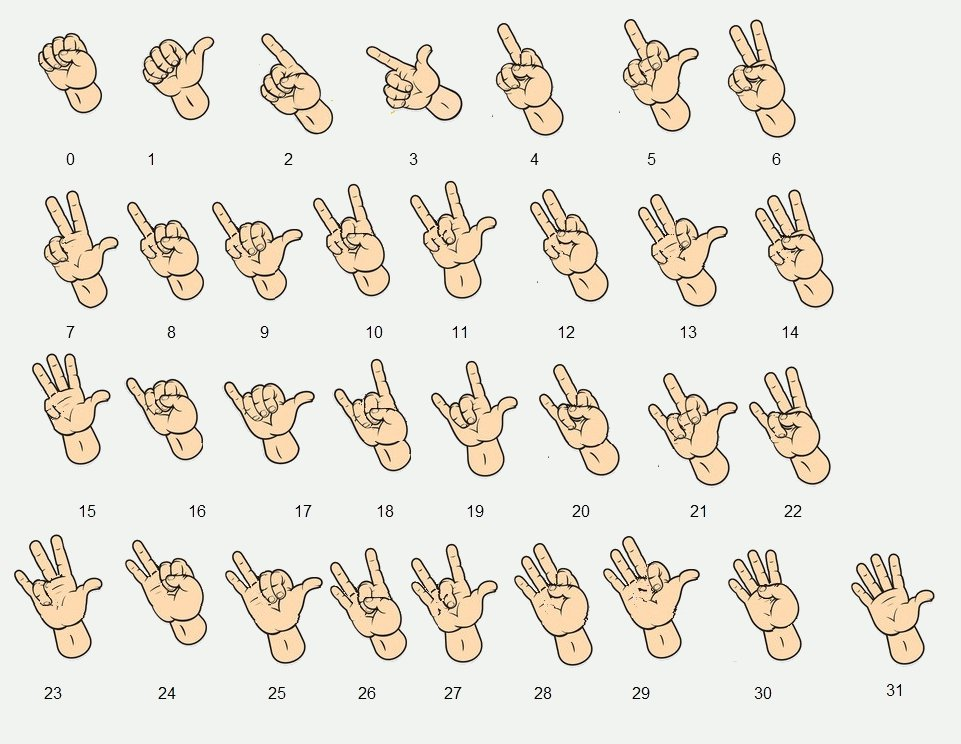
\includegraphics[width=\textwidth]{binarycount}
	\end{figure}
\end{minipage}
\end{minipage}

\begin{question}
	\begin{tasks}
		\task Wandle die Binärzahl $10001_2$ ins Dezimalsystem um. Tue dies zuerst mithilfe der Grafik oben. Überprüfe danach dein Resultat rechnerisch (wie im Beispiel oben). \grid{3.2}
		\task Wandle die Dezimalzahl $28_{10}$ mithilfe der Grafik oben ins Binärsystem um. \grid{3.2}
		\task Warum ist die Zahl $10010_2$ die Lieblingszahl von jedem Heavy Metal Fan? \grid{3.2}
	\end{tasks}
\end{question}
\begin{solution}
	\begin{tasks}
		\task $17_{10}$
		\task $11100_2$
		\task \url{https://de.wikipedia.org/wiki/Mano_cornuta}
	\end{tasks}
\end{solution}

\newpage

\begin{question}
	Wandle die Binärzahlen ins Dezimalsystem um. Gehe dabei \textit{rechnerisch} vor. Jeder Rechenschritt muss dabei klar ersichtlich sein.
	\begin{tasks}(2)
		\task $111_2$
		\task $1000011_2$
		\task $1101010_2$
		\task $100010001000_2$
	\end{tasks}
	\grid{14.2}
\end{question}
\begin{solution}
	\begin{tasks}
		\task $111_2 = 1\cdot2^2+1\cdot2^1+1\cdot2^0 = 4+2+1 = 7$
		\task $1000011_2 = 1\cdot2^6+0\cdot2^5+0\cdot2^4+0\cdot2^3+0\cdot2^2+1\cdot2^1+1\cdot2^0
		= 2^6+2+1=64+2+1=67$
		\task $1101010_2=106$
		\task $100010001000_2 = 2^{11}+2^7+2^3 = 2184$
	\end{tasks}
\end{solution}

\begin{question}
	Schreibe in \textbf{TigerJython} ein Programm, welches \textbf{Binärzahlen in Dezimalzahlen} umwandelt. Definiere im Programm eine Funktion \pythoninline{binaer_zu_dezimal(b)}, welche eine Binärzahl \pythoninline{b} als Argument entgegen nimmt, in eine Dezimalzahl umrechnet und mit return zurückgibt. Überprüfe deinen Code, indem du diesen auf die Beispiele aus der letzten Aufgabe anwendest.

	Dazu einige Tipps:
	\begin{itemize}
		\vspace{-\topsep}
		\item Schreibe die Binärzahl als String,  z.B. \pythoninline{b = '100101'}.
		\item Ein String kann dann behandelt werden wie ein Array. Mit \pythoninline{b[2]} kann man den dritten Buchstaben des Strings \pythoninline{b} auslesen. Auch kann man genau gleich mit einer for-Schleife (\pythoninline{for x in b:} \ldots) durch alle Buchstaben des Strings durchgehen. 
	\end{itemize}		
\end{question}
\begin{solution}
	\textcolor{red}{Schicke deinen Code per Teams deiner Lehrperson.}
\end{solution}

\newpage

\begin{question}
	% \textbf{Bits \& Bytes:}
	Nimmt man $8$ Bits zusammen, so erhält man ein \textbf{Byte}, zum Beispiel $1001\,1010_2$.
	Löse alle Aufgaben in dieser Aufgabe \textit{rechnerisch}. Verwende deinen Code aus der letzten Aufgabe nur, um deine Resultate zu überprüfen.
	\begin{tasks}
		\task Wieviele verschiedenen Zustände kann man mit einem einzigen Byte ausdrücken und warum?
		\grid{4.2}
		\task Mit einem Byte sollen positive ganze Zahlen inklusive $0$ ausgerückt werden. Was ist die grösste mögliche Zahl?
		\grid{5.2}
		\task Es solle nun nicht nur $1$ Byte, sondern $x$ Bytes zur Verfügung stellen. Was ist nun die grösste mögliche Zahl, die man damit darstellen kann.
		\grid{5.2}
		\task Wie viele Bytes benötigt man, um den Kontostand von Elon Musk speichern zu können? (Stand Anfangs 2021: $162$ Mia.\$)
		\grid{5.2}
	\end{tasks}
\end{question}
\cprotEnv\begin{solution}
	\begin{enumerate}[label=\alph*)]
		\item $8$ bits mit je $2$ möglichen Zuständen:
		$$2^8 = 256$$
		\item $2^8-1 = 256 - 1 = 255$ (das $-1$ braucht es, weil $0$ die kleinste Zahl ist)

		Lösungsvariante 1 im Detail (elegant): Mit $8$ Bits kann man $2^8 = 265$ Zahlen darstellen. Ist $0$ die kleinste, muss $255$ die grösste sein.

		Lösungsvariante 1 im Detail (weniger elegant):
		Die grösste Zahl ist $1111\,1111_2$. Umrechnen in Dezimalzahl ergibt $255$
		\item $2^{8x}-1$
		\item $6$ Bytes. Mit $5$ Bytes kann man maximal eine gute Milliarde darstellen (reicht nicht), mit $6$ Bytes sind es $281$ Milliarden (reicht).
	\end{enumerate}
\end{solution}

˙\newpage

Wir wissen nun, wie man Binärzahlen in Dezimalzahlen umwandelt.
Ziel dieser Aufgabe ist herauszufinden, wie der umgekehrte Schritt funktioniert: Das \textbf{Umwandeln von Dezimalzahlen in Binärzahlen.}

Dazu gibt es einen \textit{Algorithmus}, welcher wie folgt funktioniert: Starte mit der gegebenen Dezimalzahl und dividiere sie durch $2$ und notiere das Resultat sowie den Rest. Wiederhole nun diesen Schritt, allerdings startest du nun mit dem Resultat des letzten Schritts usw. Dies wiederholst du solange, bis als Resultat $0$ herauskommt. Die Binärzahl ist dann gegeben durch die Reste der Divisionen und zwar in umgekehrter Reihenfolge. Dieser Algorithmus wird der \textbf{Restwert-Algorithmus} genannt.

Schauen wir uns diesen Algorithmus für die Zahl $42_{10}$ an:
\begin{align*}
	&\text{Schritt 1:}& &42                     & &/& &2& &=& &\textcolor{blue}{21}   & &\text{Rest:}& &\textcolor{red}{0}& \\
	&\text{Schritt 2:}& &\textcolor{blue}{21}   & &/& &2& &=& &\textcolor{magenta}{10}& &\text{Rest:}& &\textcolor{red}{1}& \\
	&\text{Schritt 3:}& &\textcolor{magenta}{10}& &/& &2& &=& &\textcolor{green}{5}   & &\text{Rest:}& &\textcolor{red}{0}& \\
	&\text{Schritt 4:}& &\textcolor{green}{5}   & &/& &2& &=& &\textcolor{orange}{2}  & &\text{Rest:}& &\textcolor{red}{1}& \\
	&\text{Schritt 5:}& &\textcolor{orange}{2}  & &/& &2& &=& &\textcolor{cyan}{1}    & &\text{Rest:}& &\textcolor{red}{0}& \\
	&\text{Schritt 6:}& &\textcolor{cyan}{1}    & &/& &2& &=& &\textcolor{black}{5}   & &\text{Rest:}& &\textcolor{red}{1}&   
\end{align*}

Das Resultat ist also
$$42_{10} = \textcolor{red}{101010}_2$$

Damit man diese Rechnung auch etwas kürzer - aber doch übersichtlich - darstellen kann, bietet sich folgende Darstellung an:
\begin{table}[H]
	\centering
	\renewcommand{\arraystretch}{1.5}
	\begin{tabular}{|c|c|}
	\hline
	\textbf{42} & \\ \hline
	21 & 0 \\ \hline
	10 & 1 \\ \hline
	 5 & 0 \\ \hline
	 2 & 1 \\ \hline
	 1 & 0 \\ \hline
	 0 & 1 \\ \hline
	\end{tabular}
\end{table}

\newpage 

\begin{question}
	Wandle folgende Dezimalzahlen mit Hilfe des Restwert-Algorithmus in Binärzahlen um. Achte auf eine saubere und klare Darstellung.
 	\begin{tasks}(2)
		\task $\num{13}_{10}$
		\task $\num{19}_{10}$
		\task $\num{217}_{10}$
		\task $\num{56379}_{10}$
	\end{tasks}
	\grid{18.2}
\end{question}
\begin{solution}
	\begin{tasks}
		\task $\num{13}_{10} = 1101_2$
		\task $\num{19}_{10} = 10011_2$
		\task $\num{217}_{10} = 11011001_2$
		\task $\num{56379}_{10} = 1101110000111011_2$
	\end{tasks}

	Beispiellösung für eine der Teilaufgaben:
	\begin{table}[H]
		\centering
		\renewcommand{\arraystretch}{1.5}
		\begin{tabular}{|c|c|}
		\hline
		\textbf{13} & \\ \hline
		6 & 1 \\ \hline
		3 & 0 \\ \hline
		1 & 1 \\ \hline
		0 & 1 \\ \hline
		\end{tabular}
	\end{table}
	$$\ra 13_{10} = 1101_2$$

\end{solution}

\newpage

\cprotEnv\begin{question}
	\textbf{Implementiere den Restwert-Algorithmus in Python.} Definiere im Programm eine Funktion \pythoninline{dezimal_zu_binaer(d)}, welche eine Dezimalzahl \pythoninline{d} als Argument entgegen nimmt, in eine Binärzahl umrechnet und mit return zurückgibt. Überprüfe deinen Code, indem du diesen auf die Beispiele aus der letzten Aufgabe anwendest.
\end{question}
\begin{solution}
\end{solution}

\newpage

	
% \begin{enumerate}[label=\alph*]
% 	\item \begin{csharp}
% 		uint x = 4294967295;
% 		Console.WriteLine (x);
% 		\end{csharp}
% \end{enumerate}


% \begin{question}
% 	123
% \end{question}
% \begin{solution}
% 	\begin{python}
% 		# nur a)
% 		x = input("Gib eine ganze Zahl ein:")
% 		for i in range(x+1):
% 			print(i*i)
% 	\end{python}
% \end{solution}

% Du kennst sicher schon die folgenden Präfixe, zum Beispiel von Masseinheiten wie dem Kilogram:
% \begin{table}[H]
% 	\centering
% 	\renewcommand{\arraystretch}{1.5}
%   	\begin{tabular}{|>{\centering\arraybackslash}p{2cm}|
%   					 >{\centering\arraybackslash}p{2cm}|
%   					 >{\centering\arraybackslash}p{2cm}|
%   					 >{\centering\arraybackslash}p{2cm}|
% 					 }
% 	\hline
% 	\rowcolor[HTML]{FFCE93} 
% 	\textbf{Präfix} & \textbf{Symbol} & \textbf{Potenz} & \textbf{Dezimalzahl} \\ \hline
% 	Kilo & k & $10^3$ & \num{1000} \\ \hline
% 	Mega & M & $10^6$ & \num{1000000} \\ \hline
% 	Giga & G & $10^9$ & \num{1000000000} \\ \hline
% 	\end{tabular}
% \end{table}

% Speichergrössen werden zum Beispiel in GB

\begin{comment}

\subsubsection{Addition}

\begin{question}
	Das \textbf{schriftliche Addieren von zwei binären Zahlen} funktioniert gleich wie das schriftliche Addieren von Dezimalzahlen, welches man in der Primarschule lernt.
	\begin{tasks}
		\task Führe zum Aufwärmen die folgende Addition zweier Dezimalzahlen schriftlich aus:
		$$\num{50974}_{10} + \num{81963}_{10}$$
		\grid{5.2}
		\task Führe nun folgende Additionen schriftlich aus:
		\begin{itemize}
			\item $1100\,1100_2 + 0011\,0011_2$
			\item $1100\,1011_2 + 1010\,1110_2$
			\item $1101\,0010_2 + 1100\,0101_2$
			\item $1110\,1111_2 + 1011\,0101_2$
		\end{itemize}
		\grid{13.2}
	\end{tasks}
\end{question}
\begin{solution}
	\begin{tasks}
		\task 
			\begin{table}[H]
				\centering
				\renewcommand{\arraystretch}{1.2}
				\begin{tabular}{L@{\hspace{1cm}}*{6}{C}}
				\rowfont{\normalfont}
					&& 5&0&9&7&4\\
				+&& 8&1&9&6&3\\
				\rowfont{\footnotesize}
				&&  &1&1& & \\	\hline
				\rowfont{\normalfont}
				&1&3&2&9&3&7
				\end{tabular}
			\end{table}
		%%%		
		\task 
		\begin{itemize}
			\item $1100\,1100_2 + 0011\,0011_2 = 1111\,1111_2$
			\item $1100\,1011_2 + 1010\,1110_2 = 1\,0111\,1001$
			\item $1101\,0010_2 + 1100\,0101_2 = 1\,1001\,0111_2$
			\item $1110\,1111_2 + 1011\,0101_2 = 1\,1010\,0100_2$
		\end{itemize}
		Zweites Beispiel im Detail:
		\begin{table}[H]
			\centering
			\renewcommand{\arraystretch}{1.2}
			\begin{tabular}{L@{\hspace{1cm}}*{11}{C}}
			\rowfont{\normalfont}
			  &&1&1&0&0&1&0&1&1 \\ 
			  &&1&0&1&0&1&1&1&0 \\
			\rowfont{\footnotesize}
			  &1& & & &1&1&1& &  \\ \hline
			\rowfont{\normalfont}
			  &1&0&1&1&1&1&0&0&1  \\
			% && & & & & & & &  \\
		\end{tabular}
		\end{table}
		Letztes Beispiel im Detail:
		\begin{table}[H]
			\centering
			\renewcommand{\arraystretch}{1.2}
			\begin{tabular}{L@{\hspace{1cm}}*{11}{C}}
			\rowfont{\normalfont}
			  &&1&1&1&0&1&1&1&1 \\ 
			+ &&1&0&1&1&0&1&0&1 \\
			\rowfont{\footnotesize}
			  &&1&1&1&1&1&1&1&  \\ \hline
			\rowfont{\normalfont}
			  &1&1&0&1&0&0&1&0&0 \\
			\end{tabular}
		\end{table}
	\end{tasks}
\end{solution}



\newpage

\subsubsection{Negative Zahen \& Subtraktion}

In der Mathematik ist die Subtraktion keine eigene Operation, denn sie ist durch die Addition definiert: $a - b = a + (-b)$, oder: `Subtraktion' = `Addition der Gegenzahl'.
Damit man eine Binärzahl von einer anderen subtrahieren kann, muss man deshalb zuerst festlegen, wie man \textbf{negative Zahlen} ausdrückt.

Man könnte sich zum Beispiel darauf einigen, dass das Bit ganz links über das Vorzeichen entscheidet und der Absolutwert der Zahl durch die restlichen Bits festgelegt ist. Dann wäre $0101_2 = +5_{10}$ und $1101_2 = -5_{10}$. Dies birgt aber ein Problem: Addiert man eine Zahl mit seiner Gegenzahl, so möchte man $0$ erhalten. Dies ist mit dieser Definition aber nicht der Fall: $0101_2 + 1101_2 = 10010_2 \neq 0.$ Deshalb verwerfen wir diesen Ansatz, um negative Zahlen darzustellen.

Eine negative Zahle wird durch ihr \textbf{2er-Komplement} ausgedrückt. Dabei muss man zuerst festlegen, wieviele Bits die Zahlen haben sollen. Für 4-Bit ist das 2er-Komplement von $0101_2 = +5_{10}$ die Zahl $1011_2$. Addieren wir die beiden Zahlen, so erhalten wir $1\,0000_2$. In 4-Bit fällt die Stelle links weg und es bleibt $0000_2$ übrig.

Das 2er-Komplement bildet man wie folgt:
\vspace{-0.4cm}
\begin{itemize}
	\item Die Zahl wird in der gewünschten Anzahl Bits ausgedrückt.
	\item Dann werden alle Bits invertiert ($0 \ra 1, 1 \ra 0)$ \ldots
	\item und am Schluss $1$ dazu addiert.
\end{itemize}

Das MSB entscheidet hier also darüber, ob die Zahl positiv oder negativ ist.

\begin{figure}[H]
	\centering
	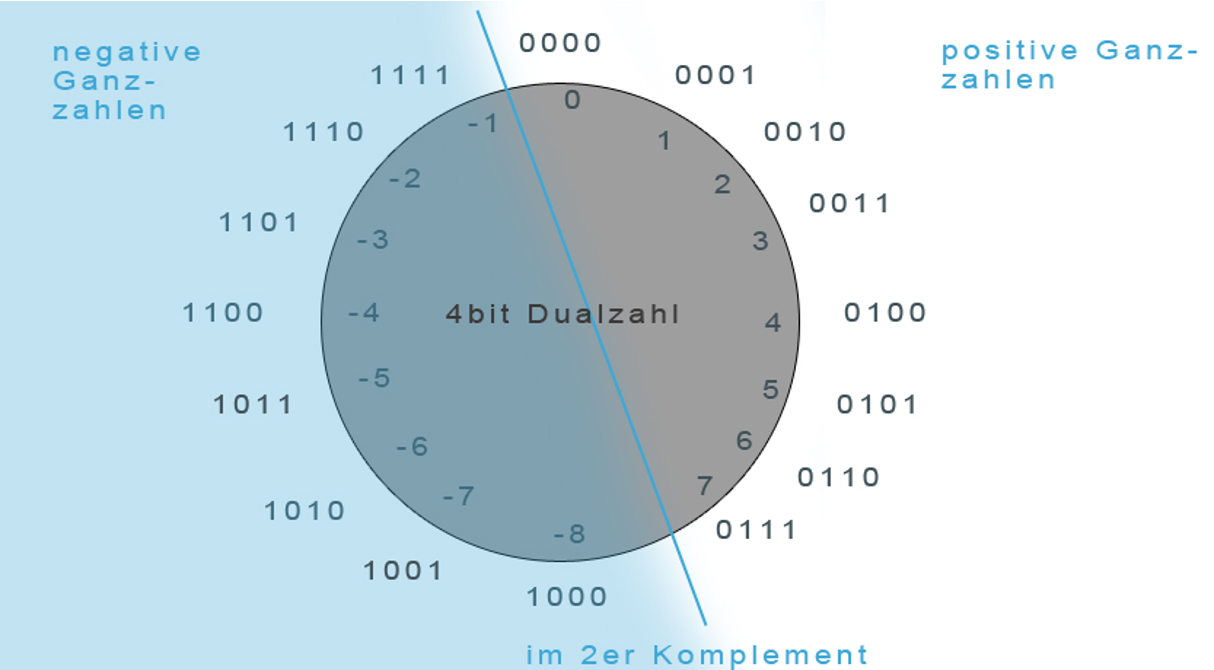
\includegraphics[width=0.9\textwidth]{2erkomplement}
\end{figure}

\newpage

\begin{question}
	\begin{tasks}
		\task Bestimme die Gegenzahl von $101101_2$ in 8-Bit.
		\task Welche negative Dezimalzahl wird durch die Zahl $1010\,1011_2$ ausgedrückt?
	\end{tasks}	
	\grid{5.2}
\end{question}
\begin{solution}
	\begin{tasks}
		\task Zahl: $0010\,1101_2$, Gegenzahl: $1101\,0011_2$
		\task $0101\,0101_2 = 85_{10}$, also $1010\,1011_2 = -85_{10}$
	\end{tasks}
\end{solution}

\begin{question}
	Führe die folgenden Subtraktionen aus. Bestimme dazu vom Subtrahend das 2er-Komplement und addiere dann die beiden Zahlen. Die einzelnen Zahlen sind als positive Zahlen zu interpretieren. Um das 2er-Komplement zu bilden, müssen sie also erweitert werden.
	\begin{tasks}
		\task $1000\,0000_2 - 0001\,1111_2$
		\task $1010\,1011_2 - 0110\,1011_2$
		\task $1111\,0010_2 - 1000\,1111_2$
	\end{tasks}
	\grid{14.2}
\end{question}
\begin{solution}
	\begin{tasks}
		\task $1000\,0000_2 - 0001\,1111_2 = 0110\,0001_{2}$
		\task $1010\,1011_2 - 0110\,1011_2 = 0100\,0000_{2}$
		\task $1111\,0010_2 - 1000\,1111_2 = 0110\,0011_{2}$
	\end{tasks}
	Zweite Aufgabe im Detail: Zwei positive 8-Bit Zahlen $\ra$ erweitere auf 9-Bit:
	\bas
	1010\,1011_2 - 0110\,1011_2
	&= 0\,1010\,1011_2 - 0\,0110\,1011_2
	\\
	&= 0\,1010\,1011_2 + 1\,1001\,0101_2
	\\
	&= 10\,0100\,0000_{2}
	\\
	&= 0\,0100\,0000_{2}
	\\
	&= 0100\,0000_{2}
	\eas
	Im zweitletzten Schritt ignorieren wir das 10. Bit, da wir mit 9-Bit zahlen gerechnet haben. Im letzten Schritt schreiben wir das Resultat als 8-Bit Zahl, da die ursprünglichen Zahlen auch als solche dargestellt wurden.
\end{solution}

\newpage

\begin{question}
	\begin{tasks}
		\task Bestimme die grösste und kleinste Zahl, die man mit 4-Bits ausdrücken kann als Binär- und Dezimalzahl.
		\grid{4.2}
		\task In C\# ist ein \textbf{\textit{int}} eine positive oder negative ganze Zahl, der insgesamt 4 Bytes zur Verfügung stehen. Was ist die grösste und kleinste Zahl, die man mit einem int darstellen kann? Bestimme als Dezimalzahl.
		\grid{5.2}
		\task Überprüfe dein Resultat aus der letzten Aufgabe direkt in C\#: Vergrösserst (verkleinerst) du die grösste (kleine) Zahl um $1$, so musst du eine Fehlermeldung erhalten.
		\task Was sind die Gemeinsamkeiten und Unterschiede zwischen den beiden Datentypen \textbf{\textit{int}} und \textbf{\textit{uint}}?
		\grid{5.2}
	\end{tasks}
\end{question}
\cprotEnv\begin{solution}
	\begin{tasks}
		\task grösste Zahl: $0111_2 = 7_{10}$, kleinste Zahl: $1000_1 = -8_{10}$
		\task 4 Bytes $=$ $32$ Bits:
			\begin{itemize}
				\item grösste Zahl: $2^{32-1} - 1 = \num{2147483647}$
				\item kleinste Zahl: $-2^{32-1} = -\num{2147483648}$
			\end{itemize}
		\task 
		\begin{itemize}
			\item Gemeinsamkeiten: beide 4 Bytes, beide für ganze Zahlen
			\item Unterschiede: \textbf{\textit{uint}} nur positive Zahlen, \textbf{\textit{int}} auch negative, dafür ist grösster \textbf{\textit{uint}} etwa doppelt so gross wie grösster \textbf{\textit{int}}
		\end{itemize}
		\task
	\end{tasks}
	\begin{csharp}
		int a;
		// kein Fehler
		a = 2147483647;
		a = -2147483648;
		Console.WriteLine(a);			
		// Fehler
		a = 2147483648;
		a = -2147483649;
		Console.WriteLine(a);
	\end{csharp}
\end{solution}

Möchte man mit besonders grossen oder kleinen ganzen Zahlen arbeiten, so kann man den Datentypen \textbf{\textit{long}} verwenden. Dieser stellt eine positive oder negative ganze Zahl in 8 Bytes dar.

\lp{
	\newpage
	\section*{LP Info}

	\subsection*{Beispiel Subtraktion} 
	
	\textbf{Lektionseinstieg}:
	Subtraktion, wobei der Subtrahend grösser ist als der Minuend:
	\bas 
	011_2 - 101_2
	= 0011_2 - 0101_2
	= 0011_2 + 1011_2
	= 1110_2
	= -0010_2
	= -010_2
	\eas
	Dies stimmt, da:
	$$011_2 - 101_2 = 3 - 5 = -2$$
	$$-010_2 = -2$$

	\subsection*{Datentypen in Python}
	
	Ein \textbf{int} hat auch 4 Bytes zur Verfügung. Grössere ganze Zahlen werden in \textbf{long}s gespeichert. Diese haben aber keine maximale Grösse sondern können beliebig gross werden (modulo Grenzen des Computers).

% 	\begin{python}
% print(type(2147483647)) # <type 'int'>
% print(type(2147483648)) # <type 'long'>
% 	\end{python}	

}

\newpage

\subsubsection{Multiplikation}

\begin{question}
	Auch die \textbf{schriftliche Multiplikation von Binärzahlen} ist analog zur derjenigen von Dezimalzahlen.
	\begin{tasks}
		\task Multipliziere zur Auflockerung zuerst folgende Multiplikation schriftlich aus:
		$$7905_{10} \cdot 3815_{10}$$
		\grid{6.2}
		\task Multipliziere nun die folgenden Binärzahlen schriftlich. Achtung: Aufpassen hier muss man mit den Überträgen am Schluss beim Aufsummieren. Ist die Summe $5$, so notiert man eine $1$ und bei der \textit{übernächsten} Stelle einen Übertrag von $1$, da $5_2 = 101_2$.
		\begin{itemize}
			% \item $1010_2 \cdot 1011_2$
			\item $1101_2 \cdot 1111_2$
			\item $1001\,0010_2 \cdot 0110\,0011_2$
			\item $1111\,1011_2 \cdot 1110\,1011_2$
			\item $1100\,1011\,0011\,1101_2 \cdot 1110\,0111\,0111\,1010_2$
		\end{itemize}
	\end{tasks}
	\grid{11.2}
\end{question}
\begin{solution}
	\begin{tasks}
		\task 
		\begin{table}[H]
			\centering
			\renewcommand{\arraystretch}{1.2}
			\begin{tabular}{@{\hspace{1cm}}*{9}{C}}
			\rowfont{\normalfont}
			7&9&0&5&$\times$&3&8&1&5 \\ \hline
			&&&&1&9&0&7&5 \\
			&&&&&&&0&$\cdot$ \\
			&&3&4&3&3&5&$\cdot$&$\cdot$ \\
			&2&6&7&0&5&$\cdot$&$\cdot$&$\cdot$ \\ \hline
			\rowfont{\footnotesize}
			&1&1& &1& & & &  \\ \hline
			\rowfont{\normalfont}
			&3&0&1&5&7&5&7&5 \\
			\end{tabular}
		\end{table}
		\task 
		\begin{itemize}
			% \item $1010_2 \cdot 1011_2 = 0110\,1110_2$
			\item $1101_2 \cdot 1111_2 = 1100\,0011_2$
			\item $1001\,0010_2 \cdot 0110\,0011_2 = 11\,1000\,0111\,0110_2$
			\item $1111\,1011_2 \cdot 1110\,1011_2 = 1110\,0110\,0110\,1001_2$
			\item $1100\,1011\,0011\,1101_2 \cdot 1110\,0111\,0111\,1010_2 = 1011\,0111\,1100\,0100\,1110\,0110\,0001\,0010_2$
		\end{itemize}
		Zweite Aufgabe im Detail:
		\begin{table}[H]
			\centering
			\renewcommand{\arraystretch}{1.2}
			\begin{tabular}{@{\hspace{1cm}}*{9}{C}}
			\rowfont{\normalfont}
			1&1&0&1&$\times$&1&1&1&1 \\ \hline
			&&&&0&1&1&1&1 \\
			&&&1&1&1&1&$\cdot$&$\cdot$ \\
			&&1&1&1&1&$\cdot$&$\cdot$&$\cdot$ \\ \hline
			\rowfont{\footnotesize}
			&&1&&1&1&&& \\
			&& &&1& &&& \\ \hline
			\rowfont{\normalfont}
			&1&1&0&0&0&0&1&1 \\
			% &&&&&&&& \\
			\end{tabular}
		\end{table}
	\end{tasks}
\end{solution}

\newpage


\begin{question}
	\textbf{Zusatzaufgabe:}
	\begin{enumerate}
		\item Schreibe eine Funktion \textit{static string BinaryAdd(string b1, string b2)}, welche zwei in Strings gespeicherten Binärzahlen addiert und das Resultat als String zurück gibt.
		\item Schreibe eine Funktion \textit{static string BinaryMult(string b1, string b2)}, welche die beiden Strings multipliziert. Dabe sollst du auch deine Funktion \textit{BinaryAdd} verwenden.
	\end{enumerate}
\end{question}
\begin{solution}
\end{solution}


\begin{question}
	\textbf{Zusatzaufgabe für TALITS:} Schreibe eine Klasse `Binary' für Binärzahlen. Diese soll beinhalten:
	\begin{itemize}
		\item Die Binärzahl soll als String gespeichert werden. Dies hat den grossen Vorteil, dass man mit beliebig grossen Zahlen arbeiten kann.
		\item Überlagerten Konstruktor: Erzeugt man ein Binary-Objekt soll man als Argument als String in binärer Form oder als Dezimalzahl (z.B. int) übergeben können. Sämtliche Umrechnungen werden selbst gemacht.
		\item Überlagerte Operatoren: Invertieren, Addieren, Subtrahieren, Multiplizieren. Sämtliche Operationen sollen mit Binärzahlen durchgeführt werden. Alle Algorithmen sollen selbst implementiert werden.
	\end{itemize}
\end{question}
\begin{solution}
	
\end{solution}

\newpage

\subsection{Hexadezimalsystem}

In der Computerwelt ist auch das \textbf{Hexadezimalsystem}, das Zahlensystem mit Basis $16$ und Nennwerten $0,1,\ldots,9,A,B,C,D,E,F$ weit verbreitet. Üblicherweise wird der Präfix \text{0x} verwendet, um Hexadezimalzahlen zu kennzeichnen.

\begin{question}
	\begin{tasks}
		\task Wandle um vom Dezimalsystem ins Hexadezimalsystem:
		\begin{itemize}
			\item $19_{10}$
			\item $\num{32768}_{10}$
			\item $\num{56379}_{10}$
		\end{itemize}
		\grid{6.2}
		\task Wandle um vom Hexadezimalsystem ins Dezimalsystem:
		\begin{itemize}
			\item \nbaseprint{0xC}
			\item \nbaseprint{0xFFFF}
			\item \nbaseprint{0xB38A}
		\end{itemize}
		\grid{6.2}
	\end{tasks}	
\end{question}
\begin{solution}
	\begin{tasks}
		\task 
		\begin{itemize}
			\item $19_{10} = \nbaseprint{0x13}$
			\item $\num{32768}_{10} = \nbaseprint{0x8000}$
			\item $\num{56379}_{10} = \nbaseprint{0xDC3B}$
		\end{itemize}
		\task
		\begin{itemize}
			\item $\nbaseprint{0xC} = 12_{10}$
			\item $\nbaseprint{0xFFFF} = 65535_{10}$
			\item $\nbaseprint{0xB38A} = 45962_{10}$
		\end{itemize}
	\end{tasks}	
\end{solution}


\begin{question}
	Zusatzaufgabe: Google und finde heraus, wofür die folgenden Zahlen in `Hexspeak' stehen.
	\begin{itemize}
		\item \nbaseprint{0xC0CAC01A}, \nbaseprint{0xADD511FE}
		\item \nbaseprint{0xDEADC0DE}
		\item \nbaseprint{0xDECAFBAD}
		\item \nbaseprint{0xFEE1DEAD}
		\item \nbaseprint{0xBADCAB1E}
	\end{itemize}
\end{question}
\begin{solution}
	\lp{
		\url{https://en.wikipedia.org/wiki/Hexspeak}
		\begin{itemize}
			\item \nbaseprint{0xC0CAC01A}, \nbaseprint{0xADD511FE}
			\item \nbaseprint{0xDEADC0DE}
			\item \nbaseprint{0xDECAFBAD}
			\item \nbaseprint{0xFEE1DEAD} (Linux Reboot)
			\item \nbaseprint{0xBADCAB1E} (Visual Studio Debugger bei externen Geräten)
		\end{itemize}
	}
\end{solution}


\newpage

\section{Gleitkommazahlen}

Das Rechnen man mit ganzen Zahlen am Computer ist relativ problemfrei. So kann man davon ausgehen, dass der Computer einem immer genaue Resultate liefert - zumindest so lange man nicht den Bereich verlässt, der von ints oder longs abgedeckt wird. Man kann nämlich mit einem int \textit{sämtliche ganzen Zahlen beschreiben}, die es im Bereich $-2147483648$ bis $2147483647$ gibt.

Bei Gleitkommazahlen, also Zahlen mit Nachkommastellen, sieht es da anders aus. Beispielsweise gibt es nur schon im Intervall zwischen $0$ und $1$ \textit{unendlich viele rationale und reelle Zahlen!} Dies führt dazu, dass Werte meist gerundet werden müssen und damit nicht exakt dargestellt werden können. Rechnet man dann mit diesen gerundeten Werten weiter, so können sich diese Ungenauigkeiten verstärken.

\subsection{Erinnerung: Wissenschaftliche Schreibweise}

Um zu verstehen, wie Gleitkommazahlen in Computern gespeichert werden, lohnt es sich, sich die \textbf{wissenschaftliche Schreibweise}, in Erinnerung zu rufen. Diese Schreibweise solltest du aus dem Mathematikunterricht kennen. In dieser Schreibweise hat eine Zahl immer die folgende Form:
$$\pm a \times 10^b$$
\begin{itemize}
	\item Die Stelle ganz links beinhaltet das \textbf{Vorzeichen} und entscheidet deshalb darüber, ob die Zahl positiv oder negativ ist.
	\item Die Zahl $a$ vor der Potenz wird \textbf{Mantisse} genannt und erfüllt die Bedingung $1\leq a < 10$. Sie ist also eine Kommazahl, wobei \textit{genau eine} Ziffer ausser $0$ vor dem Dezimalpunkt steht.
	\item Die Zahl $b$ wird \textbf{Exponent} genannt. Grosse Zahlen haben einen positiven, kleine einen negativen Exponenten. Du kannst dir vorstellen, dass der Exponent das Komma \textit{verschiebt}.
\end{itemize}
Zum Beispiel sieht die wissenschaftliche Schweibweise der Zahl $-72024$ wie folgt aus:
$$-\num{7.2024e4}$$
Gut an der wissenschaftlichen Schreibweise ist, dass sie eine Zahl \textbf{eindeutig} beschreibt. Besonders nützlich ist sie für sehr kleine und grosse Zahlen.

\begin{question}
	Bringe in die wissenschaftliche Schreibweise:
	\begin{tasks}
		\task $\num{100023}=$
		\task $\num{0.000000000932}=$
		\task $\num{613453e84}=$
	\end{tasks}
	Fun fact: Die letzte Zahl entspricht in ihrer Grössenordnung ungefähr der geschätzten Anzahl Atome im sichtbaren Teil des Universums!
\end{question}
\begin{solution}	
	\begin{tasks}
		\task $\num{100023}=\num{1.00023e5}$
		\task $\num{0.000000000932}=\num{9.32e-10}$
		\task $\num{613453e84}=\num{6.13453e89}$
	\end{tasks}
\end{solution}

\newpage

\subsection{Binäre Gleitkommazahlen}

In \eqref{equ dezimalzahl in basis und nennwerten} und \eqref{equ binaerzahl in basis und nennwerten} haben wir gesehen, wie man ganze Dezimal- und Binärzahlen durch die jeweilge Basis und ihre Nennwerte ausdrücken kann. Ganz analog kann man auch Zahlen mit Nachkommastellen ausdrücken:

\textbf{Dezimalzahl mit Nachkommastellen:}
\begin{align}
	% \label{equ Gleitkommazahl in basis und nennwerten}
	\textcolor{blue}{42.13}_{\textcolor{magenta}{10}}
	= \textcolor{blue}{4}\times \textcolor{magenta}{10}^{\textcolor{red}{1}} 
	+ \textcolor{blue}{2}\times \textcolor{magenta}{10}^{\textcolor{red}{0}} 
	+ \textcolor{blue}{1}\times \textcolor{magenta}{10}^{\textcolor{red}{-1}} 
	+ \textcolor{blue}{3}\times \textcolor{magenta}{10}^{\textcolor{red}{-2}}
\end{align}

\textbf{Binärzahl mit Nachkommastellen:}
\begin{align}
	% \label{equ Gleitkommazahl in basis und nennwerten}
	\textcolor{blue}{101.11}_{\textcolor{magenta}{2}}
	= \textcolor{blue}{1}\times \textcolor{magenta}{2}^{\textcolor{red}{2}} 
	+ \textcolor{blue}{0}\times \textcolor{magenta}{2}^{\textcolor{red}{1}} 
	+ \textcolor{blue}{1}\times \textcolor{magenta}{2}^{\textcolor{red}{0}} 
	+ \textcolor{blue}{1}\times \textcolor{magenta}{2}^{\textcolor{red}{-1}} 
	+ \textcolor{blue}{1}\times \textcolor{magenta}{2}^{\textcolor{red}{-2}}
\end{align}

Um eine Binärzahl mit Nachkommastellen im Speicher eines Computers zu speichern, bringt man diese zuerst in die wissenschaftliche Schreibweise. Im Speicher werden dann \textit{Vorzeichen, Mantisse und Exponent} gespeichert. 
Dabei ist ein Bit für das Vorzeichen und jeweils eine \textit{feste Anzahl Bits} für Mantisse und Exponent festgelegt.
Aus dieser Information kann dann die Zahl rekonstruiert werden.

% Eine Binärzahl mit Nachkommastellen wird nun wie folgt gespeichert:
% \begin{itemize}
% 	\item In einem Bit wird das \textbf{Vorzeichen} gespeichert.
% 	\item Eine feste Anzahl Bits ist für das Speichern der \textbf{Mantisse} festgelegt und
% 	\item eine feste Anzahl Bits ist für das Speichern des \textbf{Exponenten} festgelegt.
% \end{itemize}

Die wissenschaftliche Schreibweise für Binärzahlen funktioniert analog zu der für Dezimalzahlen. Beachte, dass in der Mantisse die Ziffer vor dem Punkt \textit{eine Eins} sein muss. Die einzige Ausnahme ist die Zahl $0_2$. Beim Speichern einer Zahl mit Nachkommastellen wird deshalb diese erste $1$ \textit{weggelassen} - so spart man sich ein Bit! Man sagt, dass die Mantisse \textbf{normalisiert} wird:

In Exponenten möchte man \textbf{negative Zahlen verhindern}. Man addiert zum Exponenten deshalb einen sogenannten \textbf{Bias}. Dieser Bias-behaftete Exponent nimmt dann im Normalfall Werte zwischen $1$ und $2^x-2$ an, wobei $x$ die Anzahl Bits ist. Damit kann man Exponenten zwischen $-(2^{x-1}-2)$ und $+2^{x-1}-1$ darstellen. Die beiden Sonderfälle, wo der Bias-behaftete Exponent $0$ und $2^x$ ist, werden in der Tabelle erklärt:

\begin{table}[H]
	% \small
	\centering
	\renewcommand{\arraystretch}{1.5}
	\begin{tabular}{|c|c|c|}
	\hline
	\rowcolor[HTML]{FFCE93} 
	\textbf{Exponent} & \textbf{Mantisse} & \textbf{Beschreibung} \\ \hline
	$E = 0$ & $M = 0$ & Zahl $0$ \\ \hline
	$E = 0$ & $M > 0$ &  denormalisierte Zahl (für extrem kleine Zahlen) \\ \hline
	$2^x-1 > E > 0$ & $M \geq 0$ & normalisierte Zahl (Normalfall) \\ \hline
	$E = 2^x-1$ & $M = 0$ & Unendlich \\ \hline
	$E = 2^x-1$ & $M > 0$ & keine Zahl / Not A Number (NAN) \\ \hline
	\end{tabular}
\end{table}

Diese Zahlendarstellung wird \textbf{Gleitkommadarstellung} genannt, da die Position des Kommas je nach Zahl variiert. Diese Darstellung erlaubt, im Gegensatz zu Darstellungen mit einem festen Platz für das Komma, dass man sowohl sehr grosse wie auch sehr kleine Zahlen mit hoher Genauigkeit speichern kann. Die hier beschriebene Darstellung wird durch die Norm \textbf{Norm IEEE 754} festgelegt.

\newpage

\begin{question}
	\begin{tasks}
		\task Notiere die Zahl $101.01_2$ als Dezimalzahl.
		\grid{6.2}
		\task Notiere die Zahl $0.375_{10}$ als Binärzahl. Der Algorithmus funktioniert ähnlich wie bei den ganzen Zahlen, nur muss hier in jedem Schritt mit $2$ \textit{multipliziert} werden. Anstelle vom Rest notiert man hier den Übertrag.
		\grid{9.2}
		\task Notiere die Zahl $18.4_{10}$ als Binärzahl. 
		\grid{9.2}
	\end{tasks}	
\end{question}
\begin{solution}
	\begin{tasks}
		\task $101.01_2 = 
			  1 \cdot 2^{2}
			+ 0 \cdot 2^{1}
			+ 1 \cdot 2^{0}
			+ 0 \cdot 2^{-1}
			+ 1 \cdot 2^{-2}
			= 5.25_{10}
		$
		\task 
		\begin{table}[H]
			\centering
			\renewcommand{\arraystretch}{1.5}
			\begin{tabular}{|c|c|}
			\hline
			\textbf{0.375} & \\ \hline
			(0.)750 & 0 \\ \hline
			(1.)500 & 1 \\ \hline
			(1.)000 & 1 \\ \hline
			\end{tabular}
			$$\ra 0.375_{10} = 0.011_2$$
		\end{table}
		\task
		$$18.4_{10} = 10010.0\overline{1100}$$
		Siehe detaillierte Lösung hier: \url{https://youtu.be/hHpSwBf0DCA}
	\end{tasks}	
\end{solution}

\newpage

\begin{question}
	Ziel ist es, die Zahl $101.01_2$ als \textbf{16-Bit Gleitkommazahl} darzustellen. Dabei sind folgende Anzahl Bits reserviert für:
	\begin{table}[H]
		\centering
		\renewcommand{\arraystretch}{1.5}
		\begin{tabular}{|c|c|c|c|c|c|c|c|c|c|c|c|c|c|c|c|}
		\hline
		\cellcolor{blue!25}  \phantom{bl}& 
		\cellcolor{green!25} \phantom{bl}& 
		\cellcolor{green!25} \phantom{bl}& 
		\cellcolor{green!25} \phantom{bl}& 
		\cellcolor{green!25} \phantom{bl}& 
		\cellcolor{green!25} \phantom{bl}& 
		\cellcolor{red!25}   \phantom{bl}& 
		\cellcolor{red!25}   \phantom{bl}& 
		\cellcolor{red!25}   \phantom{bl}& 
		\cellcolor{red!25}   \phantom{bl}& 
		\cellcolor{red!25}   \phantom{bl}& 
		\cellcolor{red!25}   \phantom{bl}& 
		\cellcolor{red!25}   \phantom{bl}& 
		\cellcolor{red!25}   \phantom{bl}& 
		\cellcolor{red!25}   \phantom{bl}& 
		\cellcolor{red!25}   \phantom{bl}\\ \hline
		\end{tabular}
	\end{table}
	\begin{table}[H]
		\centering
		\renewcommand{\arraystretch}{1.5}
		\begin{tabular}{|c|c|c|}
		\hline
		\cellcolor{blue!25} Vorzeichen ($1$ Bit) & 
		\cellcolor{green!25} Exponent ($5$ Bits) &
		\cellcolor{red!25} Mantisse ($10$ Bits) \\ \hline
		\end{tabular}
	\end{table}
	\begin{tasks}
		\task Notiere die Zahl zuerst in der wissenschaftlichen Schreibweise für Binärzahlen:
		\grid{3.2}
		\task Wandle nun die Zahl aus dieser Form direkt ins Dezimalzahl um. Natürlich sollst du das gleiche Resultat erhalten wie in der Aufgabe auf der vorherigen Seite.
		\grid{3.2}
		\task Bestimme (jeweils als Binärzahl):
		\begin{itemize}
			\item Vorzeichen:
			\item Exponent:
			\item Mantisse:
		\end{itemize}
		\task Welche Werte sollen der minimale und maximale Exponent haben können? Bestimme den passenden \textbf{Bias}, den man zum Exponenten hinzuaddiert.
		\grid{4.2}
		\task Normalisiere nun die Mantisse und addiere den Bias zum Exponenten:
		\begin{itemize}
			\item Vorzeichen:
			\item Exponent mit Bias:
			\item Mantisse:
		\end{itemize}
		\task Notiere nun die fertige Gleitkommazahl, so wie sie im Computer gespeichert wird.
		\grid{3.7}
	\end{tasks}
\end{question}
\begin{solution}
	\begin{tasks}
		\task $$101.01_2 = \textcolor{blue}{1.0101}_2 \cdot 2^{\textcolor{red}{2}_{10}} = \textcolor{blue}{1.0101}_2 \cdot 2^{\textcolor{red}{10}_2}$$
		\task \begin{itemize}
			\item Vorzeichen: $+$, also $0_2$
			\item Exponent: $10_2$
			\item Mantisse: $1.0101_2$
		\end{itemize}
		\task Da $5$ Bit für Exponenten:
		\begin{itemize}
			\item minimaler Exponent: $-(2^{5-1}-2) = -14$
			\item maximaler Exponent: $2^{5-1}-1 = 15$
			\item Bias: $B = 15_{10} = 01111_2$
		\end{itemize}
		\lp{
			Beachte, dass Bias $15_{10}$ und nicht $14_{10}$ sein muss, da der Bias-behaftete Exponent der kleinsten normalen Zahl $00001_2$ ist und nicht $00000_2$, da dieser Exponent die Zahl $0$ (oder eine denormalisierte Zahl) darstellt. 
		}
		\task \begin{itemize}
			\item Vorzeichen: $0_2$
			\item Exponent mit Bias: $10_2 + 01111_2 = 10001_2$
			\item Mantisse: $0101000000_2$
		\end{itemize}
		\task $$0\,10001\,0101000000$$
	\end{tasks}
\end{solution}

\newpage

\begin{question}
	\begin{tasks}
		\task Bestimme für eine $16$-Bit Gleizkommazahl die grösste und zweitgrösste Zahl, die man darstellen kann als Dezimalzahl. Was fällt dir auf?
		\grid{8.2}
		\task Bestimme die kleinste positive und von Null verschiedene $16$-Bit Gleizkommazahl, die man als normalisierte Zahl darstellen kann. Rechne sie in eine Dezimalzahl um.
		\grid{8.2}
	\end{tasks}
\end{question}
\begin{solution}
	\begin{tasks}
		\task grösste Zahl:
			\begin{align*}
				0\,11110\,1111111111
				% &= 1.1111111111_2 \cdot 2^{11110_2 - 01111_2} \\
				% &= 1.1111111111_2 \cdot 2^{01111_2} \\
				= 1.1111111111_2 \cdot 2^{15_{10}}
				= 2^{15} + 2^{14} + \ldots + 2^6 + 2^5
				= \num{65504}
			\end{align*}
			zweitgrösste Zahl:
			\begin{align*}
				0\,11110\,1111111110
				= 1.1111111110_2 \cdot 2^{15_{10}}
				= 2^{15} + 2^{14} + \ldots + 2^6 + 0 \times 2^5
				= \num{65472}
			\end{align*}
			Beachte: Es gibt zwischen diesen Zahlen einen beachtlichen Bereich, der NICHT dargestellt werden kann als $16-$Bit Zahl, zum Beispiel die Zahl \num{65500}
		\task Kleinste positive normalisierte Zahl:
		\begin{align*}
			0\,00001\,0000000000
			= 1.0000000000_2 \cdot 2^{-14_{10}}
			= 2^{-14}
			\approx \num{6.103e-5}
		\end{align*}
		Zweitkleinste positive normalisierte Zahl:
		\begin{align*}
			0\,00001\,0000000001
			= 1.0000000001_2 \cdot 2^{-14_{10}}
			= 2^{-14} + 2^{-24}
			\approx \num{6.109e-5}
		\end{align*}

	\end{tasks}
\end{solution}

\begin{question}
	Für eine Gleitkommazahl stehen insgesamt $x$ Bits zur den Exponenten zur Verfügung. Stelle eine Formel auf oder gib ein Rezept an, wie man den zugehörigen Bias berechnet:
	\grid{5.2}
\end{question}
\begin{solution}
	$$B = 2^{x-1}-1 = 011\ldots1_2$$
	% Wobei insgesamt $x-1$ Einsen notiert werden.
\end{solution}

\newpage

In C\# und vielen anderen Programmiersprachen arbeitet man primär mit zwei Typen von Gleitkommazahlen, welche folgende Genauigkeiten haben:
\begin{itemize}
	\vspace{-\topsep}
	\item \textbf{Einfache Genauigkeit} (single precision): $32$-Bit Zahlen, genannt \textbf{float}
	\begin{table}[H]
		\centering
		\renewcommand{\arraystretch}{1.5}
		\begin{tabular}{|c|c|c|}
		\hline
		\cellcolor{blue!25} Vorzeichen ($1$ Bit) & 
		\cellcolor{green!25} Exponent ($8$ Bits) &
		\cellcolor{red!25} Mantisse ($23$ Bits) \\ \hline
		\end{tabular}
	\end{table}
	\item \textbf{Doppelte Genauigkeit} (double precision): $64$-Bit Zahlen, genannt \textbf{double}
	\begin{table}[H]
		\centering
		\renewcommand{\arraystretch}{1.5}
		\begin{tabular}{|c|c|c|}
		\hline
		\cellcolor{blue!25} Vorzeichen ($1$ Bit) & 
		\cellcolor{green!25} Exponent ($11$ Bits) &
		\cellcolor{red!25} Mantisse ($52$ Bits) \\ \hline
		\end{tabular}
	\end{table}
\end{itemize}

In C\# kannst du floats und doubles wie folgt deklarieren:
\begin{csharp}
// FLOATS
float a = 7.5f; // Standardnotation, beachte den notewendigen Suffix f
float b = 1.2e6f; // wissenschaftliche Notation, e bedeutet '10 hoch'
// DOUBLES
double c = 6.7d; // doubles haben optionalen Suffix d
double d = 9.2e-6;
\end{csharp}

\begin{question}
	\begin{tasks}
		\task Bestimme die grösste Zahl, die man mit einem float darstellen kann. Der grösste double wird in einer Zusatzaufgabe behandelt.
		\grid{10.2}
		\newpage
		\task Vergewissere dich, dass man in C\# keinere grösse Zahlen mit einem float darstellen kann.
		\grid{5.2}
		\task Führe mit C\#-floats die triviale rechnung $3.5 - 3.4$ aus. Was fällt dir auf? Erkläre!
		\grid{7.2}
	\end{tasks}	
\end{question}
\begin{solution}
	\begin{tasks}
		\task $\approx \num{3.4e38}$
		\task \csharpinline{float a = 3.4e38f;} funktioninert, \csharpinline{float b = 3.5e38f;} hingegen nicht
		\task Resultat ist: $0.1000001$. Also nicht exakt, Grund: Rundungsfehler. $3.3$ und $3.4$ haben als Binärzahl ausgedrückt jeweils unendliche viele sich periodisch wiederholende Nachkommastellen. Diese müssen gerundet werden, was zu diesem Fehler führt.
	\end{tasks}
\end{solution}


\begin{question}
	\textbf{**Zusatzaufgabe (Programmieren)}: Programmiere in C\# folgende Methoden:
	\begin{tasks}
		\task Eine Methode, welche dezimale Gleitkommazahlen in binäre Gleitkommazahlen konvertiert. 
		\task Eine Methode, welche binäre Gleitkommazahlen in dezimale Gleitkommazahlen konvertiert. 
		\task Eine Methode, welche eine binäre Gleitkommazahl (gegeben als String, z.B. $11010.101$) so darstellt, wie sie in einem Computer als $16-$Bit Zahl gespeichert werden würde.
		\task Eine Methode, welche diejenige aus der letzten Teilaufgabe verallgemeinert. Neben dem String soll der Methode übergeben werden, wieviele Bits für den Exponenten und die Mantisse zur Verfügung stehen. Unter anderem muss also auch der passende Bias berechnet werden.
	\end{tasks}
\end{question}
\begin{solution}
	
\end{solution}

\newpage

\begin{question}
	\textbf{**Zusatzaufgabe (Mathe / Programmieren)}: Für eine Gleitkommazahl stehen $e$ Bits für den Exponenten und $m$ Bits für die Mantisse zur Verfügung. Es handelt sich also um eine $(e+m+1)$-Bit Gleitkommazahl.
	Finde allgemeine Formeln für die unten aufgelisteten Grössen. Notiere diese entweder in \textit{mathematischer Schreibweise} und/oder \textit{implementiere Methoden} in C\#, die die entsprechenden Werte berechnen und zurückgeben.
	\begin{tasks}
		\task grösste Zahl
		\task zweitgrösste Zahl
		\task kleinste normalisierte Zahl grösser Null
		\task zweitkleinste normalisierte Zahl grösser Null
	\end{tasks}
	\textit{Tipp:} Für die ersten beiden Aufgaben kannst du das Summenzeichen $\sum$ verwenden:
	$$\sum_{i=0}^k a_i = a_0 + a_1 + \ldots + a_k$$
	Beim Programmieren kann entspricht dies einer for-Schleife.
	\grid{16.2}
\end{question}
\begin{solution}
	\begin{tasks}
		\task Grösste Zahl: $$\sum_{i=0}^{m} 2^{2^{e-1}-1-i}$$
		\task Zweitgrösste Zahl: $$\sum_{i=0}^{m-1} 2^{2^{e-1}-1-i}$$
		\task Kleinste Zahl: $$2^{-2^{x-1}+2}$$
		\task Zweitkleinste Zahl:
		$$
		2^{-2^{x-1}+2} + 2^{-2^{x-1}+2 - m}
		= 2^{-2^{x-1}+2}(1+2^{-m})
		$$
	\end{tasks}
\end{solution}

\newpage

\begin{question}
	\textbf{**Zusatzaufgabe (Mathe)}: Schätze die Grössenordnung der grössten Zahl, die ein Double darstellen kann, ab. Alles was du dazu verwenden darft, ist dein Kopf, also keinen Computer. Im äussersten Notfall, darfst du einen einfachen Taschenrechner verwenden.
	
	Berechne dazu die Potenz, die aus dem MSB heraus geht, was $2$ hoch `eine grosse Zahl' ist, was eine sehr grosse Dezimalzahl ergibt. Ein handelsüblicher Taschenrechner ist nicht in der Lage, diese Zahl zu berechnen. Der Trick hier ist, dass du dein Wissen über Logarithmen verwendest. Dann schaffst du diese Rechnung ganz ohne Rechner. Insbesondere benötigst du die Formel für den Basiswechsel
	$$\log_a k = \f{\log_b k}{\log_b a} \,.$$
	\grid{19.2}
\end{question}
\begin{solution}
	\lp{
		Potenz aus MSB: $2^{1023}$, wollen als $10$er Potenz schreiben, also:
		$$2^{1023} = 10^x$$
		Verwende Logarithmus um $x$ zu bestimmen:
		\begin{align*}
			x &= \log_{10} 2^{1023}
			= \f{\log_2 2^{1023}}{\log_2 10}
			= \f{1023}{\log_2 10}
		\end{align*}
		$\log_2 10$ kann man grob abschätzen:
		$\log_2 10 \approx 3.3$, da $3.3^2 \approx 10$.
		Also:
		\begin{align*}
			x \approx \f{1023}{3.3} = 310
		\end{align*}
		Genauer Wert ist: $\approx 307.95$
		Die Grössenordnung der grösszen Zahl ist also: $10^{310}$
	}
	Ohne Rechner sollte man auf die Grössenordnung $10^{310}$ kommen. Die genaue Lösung ist \num{1.798e308}.

	Falls unklar, bespreche deine Lösung mit der Lehrperson.
\end{solution}

% floats und Doubles

% Genauigkeit

% Rundungsfehler

% \textbf{Beispiel:} 
% \begin{enumerate}
% 	\item 
% 	\item 
% 	\item Der Exponent als Binärzahl ist $\textcolor{red}{10}_2$.
% \end{enumerate}

% \newpage




% \begin{question}
% 	??? Im Elektronikkurs hast du gelernt, wie ein Rechner zwei Binärzahlen addiert. Diese Schaltung hast du auch auf EveryCircuit implementiert. Wie würdest du nun vorgehen, um zwei Binärtzahlen zu \textit{multiplizieren}? Erkläre Schritt für Schritt.
% \end{question}
% \begin{solution}
% \end{solution}


%------------------------------------ \\
%------------------------------------
%------------------------------------
%------------------------------------
%------------------------------------
\end{comment}
%\newpage
% SOLUTIONS
%\section*{Lösungen}
%\printsolutions

\end{document}


